\documentclass[10pt,landscape]{article}
\usepackage{multicol}
\usepackage{calc}
\usepackage{ifthen}
\usepackage[landscape]{geometry}
\usepackage{hyperref}
\usepackage{amsmath}
\usepackage{graphicx}

% To make this come out properly in landscape mode, do one of the following
% 1.
%  pdflatex latexsheet.tex
%
% 2.
%  latex latexsheet.tex
%  dvips -P pdf  -t landscape latexsheet.dvi
%  ps2pdf latexsheet.ps


% If you're reading this, be prepared for confusion.  Making this was
% a learning experience for me, and it shows.  Much of the placement
% was hacked in; if you make it better, let me know...


% 2008-04
% Changed page margin code to use the geometry package. Also added code for
% conditional page margins, depending on paper size. Thanks to Uwe Ziegenhagen
% for the suggestions.

% 2006-08
% Made changes based on suggestions from Gene Cooperman. <gene at ccs.neu.edu>


% To Do:
% \listoffigures \listoftables
% \setcounter{secnumdepth}{0}


% This sets page margins to .5 inch if using letter paper, and to 1cm
% if using A4 paper. (This probably isn't strictly necessary.)
% If using another size paper, use default 1cm margins.
\ifthenelse{\lengthtest { \paperwidth = 11in}}
	{ \geometry{top=.5in,left=.5in,right=.5in,bottom=.5in} }
	{\ifthenelse{ \lengthtest{ \paperwidth = 297mm}}
		{\geometry{top=1cm,left=1cm,right=1cm,bottom=1cm} }
		{\geometry{top=1cm,left=1cm,right=1cm,bottom=1cm} }
	}

% Turn off header and footer
\pagestyle{empty}
 

% Redefine section commands to use less space
\makeatletter
\renewcommand{\section}{\@startsection{section}{1}{0mm}%
                                {-1ex plus -.5ex minus -.2ex}%
                                {0.5ex plus .2ex}%x
                                {\normalfont\large\bfseries}}
\renewcommand{\subsection}{\@startsection{subsection}{2}{0mm}%
                                {-1explus -.5ex minus -.2ex}%
                                {0.5ex plus .2ex}%
                                {\normalfont\normalsize\bfseries}}
\renewcommand{\subsubsection}{\@startsection{subsubsection}{3}{0mm}%
                                {-1ex plus -.5ex minus -.2ex}%
                                {1ex plus .2ex}%
                                {\normalfont\small\bfseries}}
\makeatother

% Define BibTeX command
\def\BibTeX{{\rm B\kern-.05em{\sc i\kern-.025em b}\kern-.08em
    T\kern-.1667em\lower.7ex\hbox{E}\kern-.125emX}}

% Don't print section numbers
\setcounter{secnumdepth}{0}


\setlength{\parindent}{0pt}
\setlength{\parskip}{0pt plus 0.5ex}


% -----------------------------------------------------------------------

\begin{document}

\raggedright
\footnotesize
\begin{multicols}{3}


% multicol parameters
% These lengths are set only within the two main columns
%\setlength{\columnseprule}{0.25pt}
\setlength{\premulticols}{1pt}
\setlength{\postmulticols}{1pt}
\setlength{\multicolsep}{1pt}
\setlength{\columnsep}{2pt}

\begin{center}
     \Large{\textbf{6.006 Cheat Sheet (shreyask)}} \\
\end{center}

\section{Recurrences}
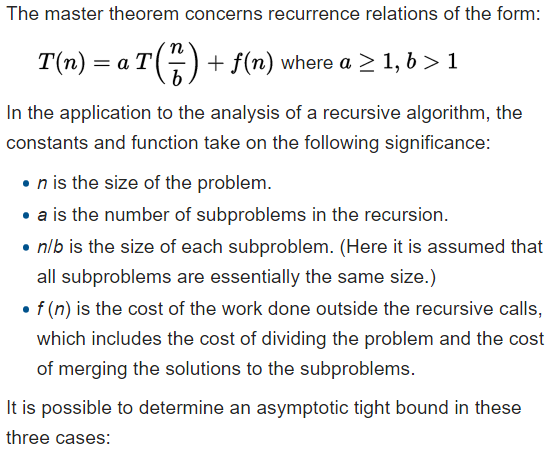
\includegraphics[scale=0.5]{mt1}
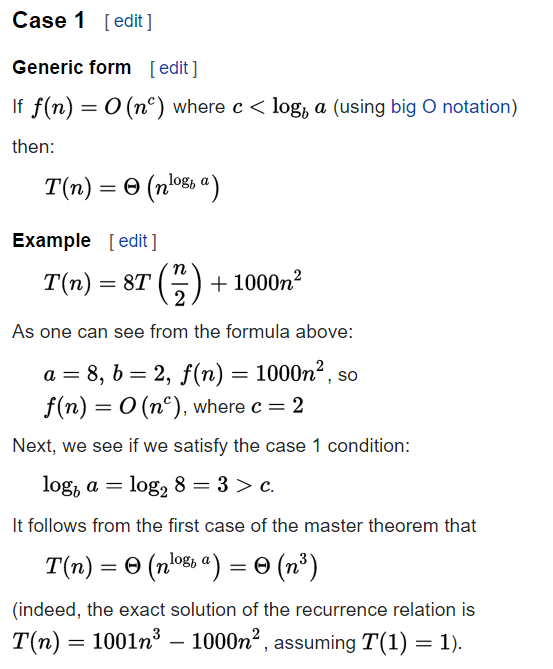
\includegraphics[scale=0.5]{mt2}
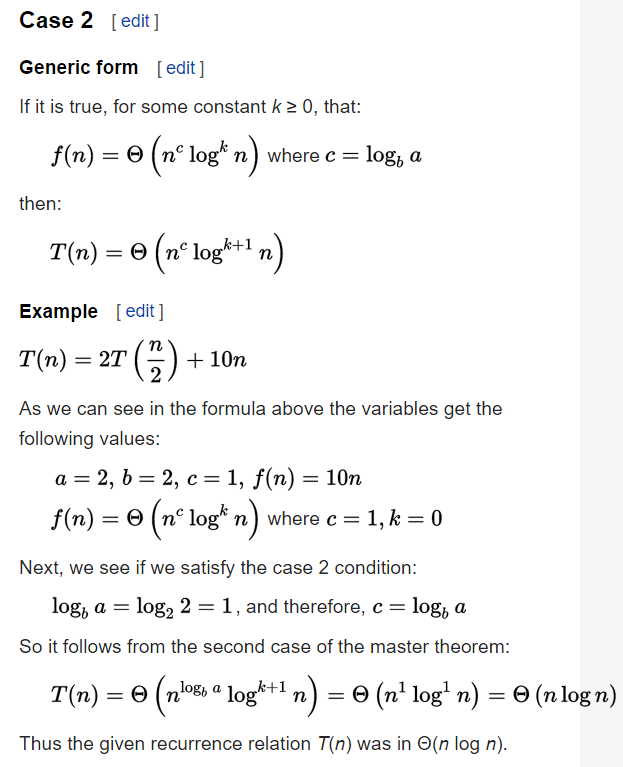
\includegraphics[scale=0.5]{mt3}
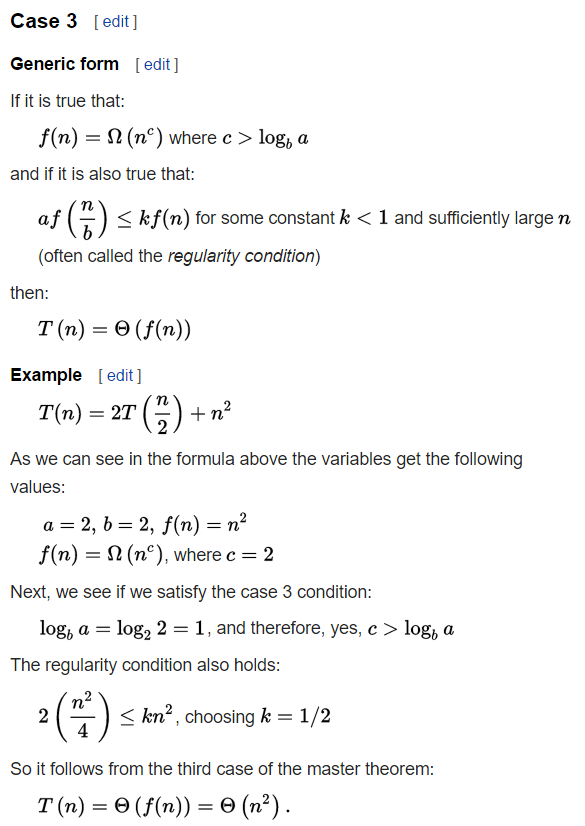
\includegraphics[scale=0.5]{mt4}

\section{Heaps}
\newlength{\MyLen}
\settowidth{\MyLen}{\texttt{letterpaper}/\texttt{a4paper} \ }

\textbf{root of tree} is $i = 0$ \\
\textbf{parent(i)} $ = i/2$, \textbf{left(i)} $ = 2i$, \textbf{right(i)} $ = 2i + 1$ \\
\textbf{max-heap prop:} the key of the node is $\geq$ the keys of its children. \\
max height of $\log n$, almost binary tree \\
\textbf{max-heapify:} assumes the left and right subtrees are maxheaps. look at both children, if higher than both: stop, else exchange from the larger children. Run maxheapify again on the same element in new position. $O(\log n)$. \\
\textbf{build-heap:} start $n/2$ and go down till the first element and call max-heapify on every element. $O(n)$. \\
\textbf{complexities:} find-max $O(1)$, delete-max $O(\log n)$, insert $O(\log n)$, decrease-key, $O(\log n)$, merge, linear.

\section{Binary Search Tree}
Useful for searching+inserting stuff. \\
Each parent has access to child, each child to parent. Left sub-tree is less than parent, right sub-tree is greater. \\
Everything $O(n)$ worst, $O(\log n)$ average \\
\textbf{insert:} search but when reach leaf insert left or right. $O(h)$\\
\textbf{find-min:} go till the left leaf or right leaf.\\
\textbf{in-order traversal:} \\
recursively iterate through left subtree, print root, recursively iterate through right subtree.

\section{AVL}
\subsection{Description of Rotations and Stuff}
Tree is balanced is $h = O(\log n)$ \\
\textbf{height of tree:} longest path from root to leaf \\
\textbf{height of node:} longest path from that node to a leaf, recursively $h(node) = max(h(left), h(right)) + 1$. The null pointers at the end of the leaves are height -1. \\
AVL Trees need the heights of left and right children of every node to differ by at most 1. \\
\textbf{AVL Insert:} \\
1. Simple BST insert \\
2. Fix AVL property from changed node up \\

Rotation changes order of nodes and stuff in constant time and maintains the BST property and the in-order order. Rotation is done at the highest unbalanced node first.
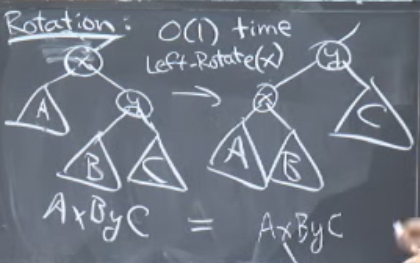
\includegraphics[scale=0.5]{left_rot}

\subsection{Proof That Difference of 1 is balanced}
$N_h$ is the minimum number of nodes that's possible of height $h$. Since the two sub trees differ by height 1,
\begin{align*}
N_h = 1 + N_{h-1} + N_{h-2} \\
> 1 + 2 N_{h-2} \\
> 2 N_{h-2} \\
= \Theta(2^{n/2}) \\
\implies h < 2 \log n
\end{align*}
\subsection{Practically Useful Stuff}
Everything in $O(\log n)$ time. Access, Search, Insertion, Deletion, Find-Max, Find-Min, Successor, Predecessor and stuff. (Cause height is maintained.)

\section{Search Bound}
\textbf{Decision Tree:} any comparison algorithm can be viewed as a tree of all possible comparisons and their outcomes and resulting answer. \\
For searching, tree is binary and must have at least $n$ leaves for each answer. Height has to be at least $\log n$

\section{Comparison Sort Lower Bound}
Decision tree is binary, number of leaves is greater than number of possible answers, which is $n!$. Height $> \log n! \implies $ Height $ > O(n \log n)$

\section{Cheaty Sorts}
\subsection{Counting Sort}
Allocate memory with the number of keys with zeros. Go through given array and update the counts in the count array. Cumulative frequencies and then place from last to first in that spot. \\
$O(n + k)$ where k the maximum value an element can take.
\subsection{Radix Sort}
Execute stable counting sort from MSB to LSB. $O(wN)$. $w$ is the number of bits in a word. 

\section{Python Costs}
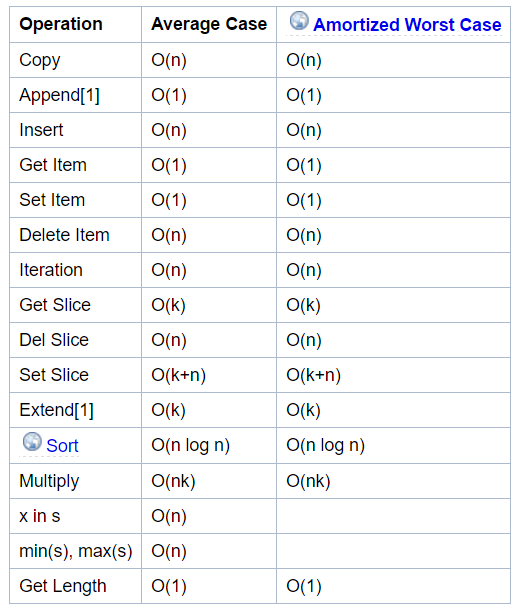
\includegraphics[scale=0.4]{costs}

\section{Hash Tables}
Pre-Hashing, whatever key we have, we convert to non-negative integer by just taking the binary representation of that object $\to$ integer.
\textbf{Chaining} if collision, store as a list. Worst case $O(n)$, any hashing. But randomized? \\
\textbf{SUHA}: each key is equally likely to be hashed to any slot of the table, independent of each other.\\
\textbf{Proof of Constant Time:}
expected length of chain $n/m = \alpha$ load factor. 
$n$ is keys, $M$ slots.
\begin{align*}
collisions = \frac{N(N-1)}{2} \frac{1}{M} \\
P(collision) = 1/m \\
P(query \ correct) = (1-1/m)^{n-1}
\end{align*}
\section{Random Useful Stuff}
\begin{align*}
f(n) = \sum_{x=1}^{n} \log x = \Theta(n \log n)
\end{align*}
Only heap sort isn't stable. \\
Only insertion and heap is in place. \\




\rule{0.3\linewidth}{0.25pt}
\scriptsize

Copyright \copyright\ 2014 Winston Chang

\href{http://www.stdout.org/~winston/latex/}{http://www.stdout.org/$\sim$winston/latex/}


\end{multicols}
\end{document}
